%%%%%%%%%%%%%%%%%%%%%%%%%%%%%%%%%%%%%%%%%
% fphw Assignment
% LaTeX Template
% Version 1.0 (27/04/2019)
%
% This template originates from:
% https://www.LaTeXTemplates.com
%
% Authors:
% Class by Felipe Portales-Oliva (f.portales.oliva@gmail.com) with template 
% content and modifications by Vel (vel@LaTeXTemplates.com)
%
% Template (this file) License:
% CC BY-NC-SA 3.0 (http://creativecommons.org/licenses/by-nc-sa/3.0/)
%
%%%%%%%%%%%%%%%%%%%%%%%%%%%%%%%%%%%%%%%%%

%----------------------------------------------------------------------------------------
%	PACKAGES AND OTHER DOCUMENT CONFIGURATIONS
%----------------------------------------------------------------------------------------

\documentclass[
	12pt, % Default font size, values between 10pt-12pt are allowed
	%letterpaper, % Uncomment for US letter paper size
	%spanish, % Uncomment for Spanish
]{fphw}

% Template-specific packages
\usepackage[utf8]{inputenc} % Required for inputting international characters
\usepackage[T1]{fontenc} % Output font encoding for international characters
\usepackage{mathpazo} % Use the Palatino font

\usepackage{graphicx} % Required for including images

\usepackage{booktabs} % Required for better horizontal rules in tables

\usepackage{listings} % Required for insertion of code

\usepackage{enumerate} % To modify the enumerate environment

\usepackage{leadsheets}

\usepackage{xcolor}

\usepackage{float}

\usepackage{caption}
\captionsetup[figure]{font=small}

%----------------------------------------------------------------------------------------
%	ASSIGNMENT INFORMATION
%----------------------------------------------------------------------------------------

\title{Homework \#2 - Automatic Chord Recognition} % Assignment title

\author{Matteo Pettenò - Marco Viviani} % Students name

\date{December 23th, 2021} % Due date

\institute{Politecnico di Milano} % Institute or school name

\class{Computer Music - Representations and Models} % Course or class name

\professor{Clara Borrelli} % Professor or teacher in charge of the assignment

%----------------------------------------------------------------------------------------

\begin{document}

\maketitle % Output the assignment title, created automatically using the information in the custom commands above

%----------------------------------------------------------------------------------------
%	ASSIGNMENT CONTENT
%----------------------------------------------------------------------------------------

\section*{Introduzione}

In this report we analyze step by step the code implemented in the attached \emph{Jupyter Notebook} trying to answer the questions asked for this homework. Along with the reading of this report, please make sure to check out code comments in the notebook. The first cells of the notebook are used to initialize the context and the parameters of the algorithm.

\subsection*{Context initialization}
In order to optimize the code for automation and readability, in this section we initialize a dictionary that contains all the details of the songs used in the experiment (\emph{Corpus}). The chord labels are generated here too.

\subsection*{Parameters configuration}
In this cell we declare and set to a default value all the template-based chord recognition algorithm's parameters. This approach allows us to centralize the management of the algorithm's behavior, making it easier to evaluate once implemented.

\section*{\color{red}Question 1}

\begin{problem}
	\textbf{Implement the template based chord recognition algorithm.}
\end{problem}

\subsection*{\color{blue}Answer}

A chord recognition algorithm is composed by two steps. In the first step, the audio track is cut into frames that are transformed into a feature vector. This is usually done by using chroma-based audio features, which contain the tonal information of the audio signal.
In the second step, pattern matching techniques are used to map each feature vector to a set of predefined chord models. The best fit determines the chord label assigned to the given frame.

\begin{figure}[H]
 \centering
 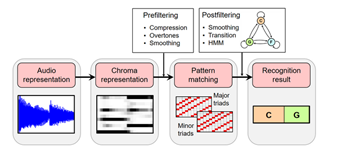
\includegraphics[scale=1]{./images/1_template_based_pipeline.png}
 \caption{Template-Based Chord Recognition Pipeline}
\end{figure}


\subsection*{Features processing functions}

In this section of the code all the functions that will be useful to implement features processing are defined. To improve the chord recognition results, in fact, additional enhancement techniques are applied either before the pattern matching step (\emph{prefiltering}) or after the pattern matching step (\emph{postfiltering}). In our implementation we only make use of prefiltering operations such as features compression, normalization, smoothing and downsampling.

\begin{enumerate}
	\item \verb|compress_feature_sequence| - This function takes in input the sequence of features and applies compression in a logarithmic fashion.
	\item \verb|normalize_feature_sequence| - This function normalizes the columns of a feature sequence. The  normalization consists in choosing a norm and then to replace each n-feature vector  by $x/p(x)$. By doing this, each chroma vector is replaced with its normalized version.  The normalization is possible only if $p(x)\neq0$, but sometimes is possible that it leads to random chroma values. This usually happens during long pauses and moments of silence, when $p(x)$ is almost equal to zero. The solution is to replace (under a certain threshold of $p(x)$) the vector $x$  by an uniform one (usually of norm one) instead of dividing by $p(x)$. In the function exactly this steps are implemented. Normalization will be used also in post filtering in order to normalize the chord similarities.
	\item \verb|smooth_feature_sequence| - Sometimes problems arise in the algorithm's pattern matching phase if the chromagrams are too detailed. A possible solution is to apply smoothing artifacts in the pre-processing step. Let \(X=(x_1,x_2,...,x_N)\) be a feature sequence with $x_n \in \mathbb{R}^k$ for $\in[1:N]$, and let be $w$ a rectangular window of length $L$. Smoothing is achieved by a convolution between the feature sequence and the window (also called kernel). As applying temporal smoothing can be regarded as bandwise lowpass filtering, the result is a smoothed feature sequence in which fast temporal fluctuations are attenuated.
	\item \verb|downsample_feature_sequence| - In order to increase the efficiency of the next processing steps this function allows to downsample the feature rate by a factor $D$ (usually much smaller than the window length $L$).
\end{enumerate}

\subsection*{Template-based chord recognition steps}

Next we define a function for each step performed by the template-based chord recognition algorithm.

\begin{enumerate}
	\item \verb|load_audio| - Loads the \emph{WAV} file.
	\item \verb|chroma_representation| - Computes (and eventually compresses) STFT-based chroma features.
	\item \verb|generate_triads_templates| - Generate chord templates for major and minor triads. This function takes no input and returns the matrix containing the chord templates as columns. Every column will be a binary vector representing the template for every minor or major chord.
	\item \verb|pre_processing| - The aim of this function is to \emph{pre-process} the features used in the algorithm. If needed, it normalizes, smooths and downsamples the chroma features and triads template with the previous defined functions.
	\item \verb|pattern_matching| - Compute the similarity matrix that compares predicted chroma features and triads template models. The similarity measure used here is the inner product between two vectors defined as:
	\begin{equation}
		s(x,y)=\frac{\langle x,y\rangle}{(||x||*||y||)}
	\end{equation}
Since our vectors contain only positive values, we have that $s(x,y)\in[0,1]$.
	\item \verb|post_processing| - Apply features \emph{post-processing}. As mentioned above, this phase must not be confused with the concept of \emph{post-filtering}: here we do not carry out any post-filtering operations, but we simply normalize the similarity matrix.
	\item \verb|recognition_result| - Returns a list containing the chord labels that maximize the similarity between the templates and the feature vectors.
\end{enumerate}

\subsection*{Template-based chord recognition implementation}

Here we answer the question with the actual template-based chord recognition algorithm implementation: the function \verb|compute_template_based_chord_recognition| receives as input the path to a \emph{WAV} file, calls the step functions defined above and returns a list where each element is the predicted chord label for the time frame n and other useful information.

\subsection*{Let It Be - Perform template-based chord recognition and plot results}

Then we perform the algorithm for the file \verb|Beatles_LetItBe.wav| and plot the results.

\begin{figure}[H]
 \centering
 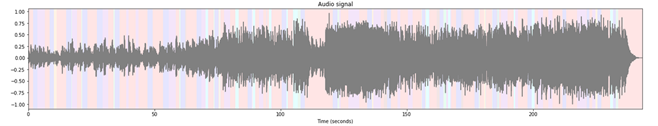
\includegraphics[scale=1]{./images/1_audio_signal.png}
 \caption{Audio Signal}
\end{figure}

\begin{figure}[H]
 \centering
 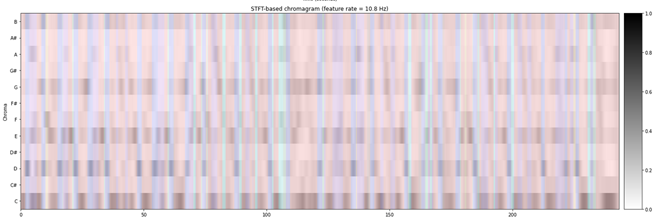
\includegraphics[scale=1]{./images/1_stft_chromagram.png}
 \caption{STFT-based Chromagram}
\end{figure}

\begin{figure}[H]
 \centering
 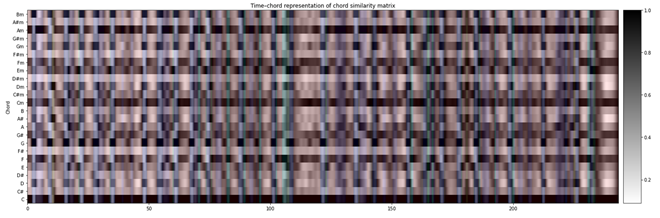
\includegraphics[scale=1]{./images/1_chord_similarity.png}
 \caption{Chord Similarity Matrix}
\end{figure}

\begin{figure}[H]
 \centering
 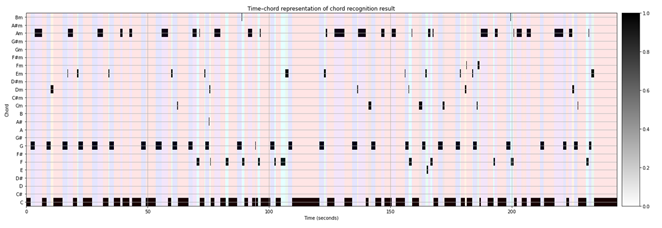
\includegraphics[scale=1]{./images/1_recognition_results.png}
 \caption{Chord Recognition Results}
\end{figure}

%----------------------------------------------------------------------------------------
\newpage
\section*{\color{red}Question 2}

\begin{problem}
	\textbf{Write a function to load and preprocess a reference annotation (or ground truth) file, saved in \emph{CSV} format.}
\end{problem}

\subsection*{\color{blue}Answer} We represent reference annotations in three formats:
\begin{itemize}
	\item \verb|segment_annotation_seconds| - This is the format given in the \emph{CSV} reference file. Each annotation is specified as a triple $(start\_seconds, end\_seconds, \lambda)$ where start and end time are given in seconds while $\lambda$ is the chord label.
	\item \verb|segment_annotation_indices| - This is an intermediate format between segment/frames conversion. Also here each annotation is defined by a triple $(start, end, \lambda)$, but start end end are defined as:
	\begin{center}
		\verb|start_index = int(np.round(start_seconds * chroma_feature_rate))|
        \verb|end_index = int(np.round(end_seconds * chroma_feature_rate))|
	\end{center}	
They represent the first and the last frame's index for the chord label $\lambda$.
	\item \verb|frame_labels_sequence| - This is our target format. It is no more defined as a tuple but as a list in which the $n$th element is che chord label for the $n$th frame.
\end{itemize}

\subsection*{Ground truth processing functions}

Now we describe the functions implemented in order to read, convert and normalize the reference \emph{CSV} file.

\begin{enumerate}
	\item \verb|read_csv| - Uses \emph{Pandas} library to read the \emph{CSV} file and returns annotations in a segment-based fashion with segments given both in indices and seconds.
	\item \verb|convert_segment_annotations| - Converts a segment-based annotation (given in indices) in the frame-wise format. It is important to notice that sometimes the frame-based sequence has to be padded or cutted in order to match the length of the recognized sequence.
	\item \verb|normalize_chord_labels| - Implements the reduction strategy for the chord labels in the given segment-based annotation sequence. Enharmonic equivalence is handled by a simple replace, while other normalizations are performed using Python's regular expressions (\emph{regex}). Half-diminished and diminished chords are considered minor chords, while suspended chords are labeled as major. The third regex performs reduction for slash chords.
\end{enumerate}

\subsection*{Ground truth reading implementation}

Finally we define the function \verb|read_ground_truth| that takes as input a path to a reference annotation \emph{CSV} file and returns the frame-wise chord labels list. Actually we can find other data in the output of this routine which are useful for the visualization of the reduction strategy.

\subsection*{Let It Be - Perform ground truth reading}

In conclusion we perform and test the ground truth reading for the file \verb|Beatles_LetItBe.csv| and plot the results.

\begin{figure}[H]
 \centering
 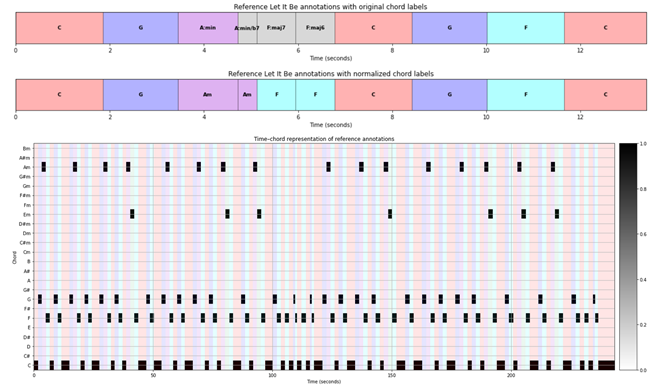
\includegraphics[scale=1]{./images/2_reference_annotations.png}
\end{figure}

%----------------------------------------------------------------------------------------
\newpage
\section*{\color{red}Question 3}

\begin{problem}
	\textbf{Propose a metric for evaluating the template based chord recognition algorithm.}
\end{problem}

\subsection*{\color{blue}Answer}

A metric is a value that tells us how good is the algorithm in performing chord recognition.
In order to define the metric we refer to a chroma sequence $X=(x_1,x_2,…,x_N)$ and to a set $\Lambda :=[$\writechord{C}, \writechord{C#},…, \writechord{B}, \writechord{Cm}, \writechord{Cm#},…, \writechord{Bm}$]$ of major and minor chords reference. Considering the set product $X \times \Lambda$, the predicted label ({n, $\lambda_n$) is called a true positive (\emph{TP}) in the case that the label is correct ($\lambda_n$=$\lambda_n^{Ref}$). Otherwise, (n, $\lambda_n$) is called a false positive (\emph{FP}) and (n, $\lambda_n^{Ref}$) a false negative (\emph{FN}). All other items are called true negative (\emph{TN}). We can define three metrics as Precision ($P$), Recall ($R$) and F-measure ($F$):

\begin{equation}
	P = \frac{\#TP}{\#TP+\#FP}
\end{equation}
\vspace{7pt}
\begin{equation}
	R = \frac{\#TP}{\#TP+\#FN}
\end{equation}
\vspace{7pt}
\begin{equation}
	F = \frac{2*P*R}{P+R}
\end{equation}
\vspace{7pt}

It is important to notice that since we have one label per frame in the reference as in the estimation the equality $\#FP=\#FN$ holds: this implies that the accuracy coincides with precision, recall, and F-measure ($P=R=F$) and it is because of this that we only compute and use the precision as our metric.

\subsection*{Metric evaluation implementation}

The function \verb|read_ground_truth| computes the precision metric as per above definition. It takes as inputs the binary time-chord matrix representation of the reference chords label sequence and the binary chord max-similarity matrix. \emph{\#TP} is obtained by logical and between the inputs while \emph{\#FP} and \emph{\#FN} are computed by difference.

\subsection*{Let It Be - Perform metric evaluation}

With the results obtained in \emph{Question 1} and \emph{Question 2} we now perform the algorithm evaluation for the song Beatles' song \emph{Let It Be}.

\begin{figure}[H]
 \centering
 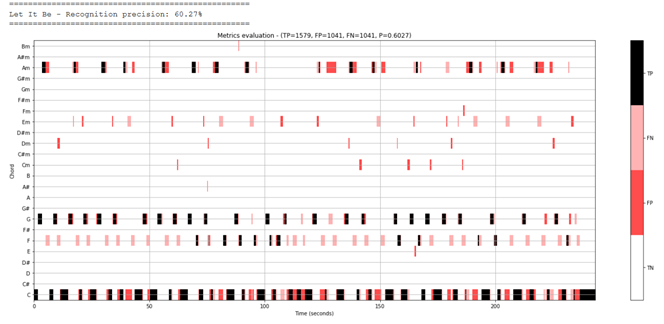
\includegraphics[scale=1]{./images/3_let_it_be_metrics.png}
 \caption{Let It Be - Metrics Evaluation}
\end{figure}

Running the algorithm with the default parameters gives us a recognition precision of \emph{60.27\%}. The visualization plotted with \emph{libfmp} plays an important role in the analysis of the evalutation. As \emph{Figure 6} shows, there are many sudden jumps between chord labels: in particular, the algorithm fails when recognize the \writechord{F} chord and this is due to the fact that in the reference annotation it is marked as \writechord{Fmaj7} which has three of its four tones in common with \writechord{Am} or \writechord{Dm} and this leads to chord ambiguities. Also we can find mistakes in the transitions between chords: this can be optimized by setting the correct STFT window length based on avarage chord transition time.

\begin{problem}
	Can you imagine a musically informed strategy that weights diferently mismatch errors of
the chord recognition algorithm?
\end{problem}

\subsection*{\color{blue}Answer}

One possible method could be the implementation of an algorithm that is no longer based only on the matching between spectral templates and template models. 
This was done instead with the template based approach.
One idea could be to make the system "musically informed", ie that knows which are the most probable changes between one chord and another.
This could be done with a code able to distinguish the tonality of the piece. 
In fact, if we know the key of the piece, the number of more probable chords would be significantly reduced. Under these assumptions, perhaps it would be necessary to introduce some mathematical instrument of the probabilistic field. 
In this regard we propose some algorithm based on transition probabilities and on Markov chains/matrices. Under these consideration we would expect a better precision in estimating the chords.

%----------------------------------------------------------------------------------------
\newpage
\section*{\color{red}Question 4}

\begin{problem}
	\textbf{Compute the proposed metric for the remaining 3 songs.}
\end{problem}

\subsection*{\color{blue}Answer}

Computing the proposed metric and averaging the results yields a mean precision of \emph{60.48\%}. The following figures visualize the results for each song.

\begin{figure}[H]
 \centering
 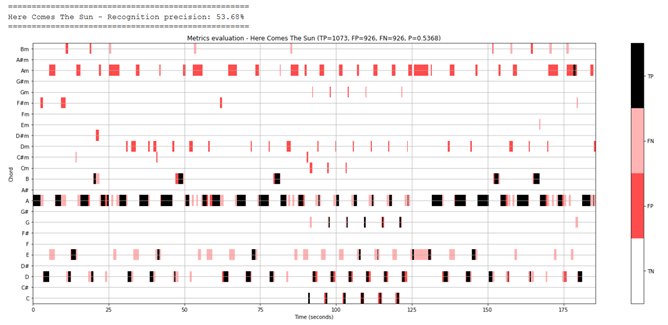
\includegraphics[scale=1]{./images/4_here_comes_the_sun_metrics.png}
 \caption{Here Comes The Sun}
\end{figure}

\begin{figure}[H]
 \centering
 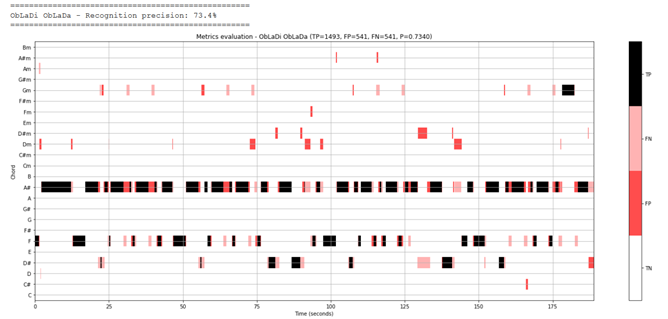
\includegraphics[scale=1]{./images/4_obladi_oblada_metrics.png}
 \caption{ObLaDì ObLada}
\end{figure}

\begin{figure}[H]
 \centering
 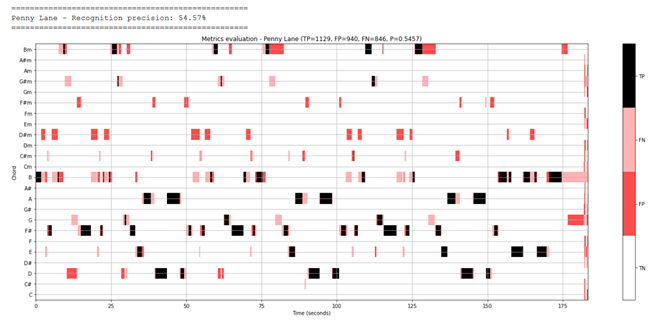
\includegraphics[scale=1]{./images/4_penny_lane_metrics.png}
 \caption{Penny Lane}
\end{figure}

%----------------------------------------------------------------------------------------
\newpage
\section*{\color{red}Question 5}

\begin{problem}
	\textbf{Analyse how algorithm parameters affect the performance of the templated based chord recognition algorithm.}
\end{problem}

\subsection*{\color{blue}Answer}

To be efficient we automated the parameter performance test: once defined the \verb|parameters_values| dictionary containing the parameters and the three values to be tested, for each of them we iterate over each song in the \verb|songs_dictionary| and overwrite the corresponding global parameter identified thanks to Python's \verb|globals()| function.
Then chords recognition, ground truth reading and metrics evaluation are performed and the outputs saved in the \verb|songs_dictionary| to allow plotting at the end.

\subsection*{Smooth filter length}

The first parameter we tested is the window length of the smooth filter. We considered the following values [0, 30, 60]: we can see an increase in accuracy up to $L=30$ and then a substantial settlement with a slight decrease. The graphs have similar trends.
We can deduce that around the value $L=30$ the precision of our algorithm will be higher. However to further increase accuracy it is necessary to set the best values for the other algorithm parameters as well.

\begin{figure}[H]
 \centering
 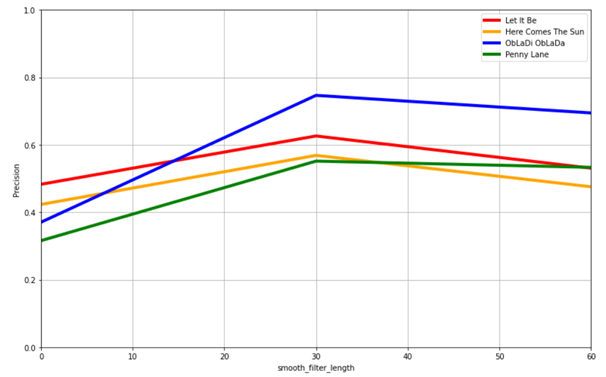
\includegraphics[scale=1]{./images/5_smooth_precision.png}
 \caption{Smooth filter length}
\end{figure}

\subsection*{Downsampling factor}

The default parameters configuration provide a smoothing of the features with a window of length $L=41$. We tested how the downsampling of the smoothed features affect the algorithm performance. Taking into account [0, 10, 100] as values ($D=0$ means no downsampling) we observe that the more the downsampling factor is increased, the more you reduce the feature rate and the less you read the harmonic content (in larger steps). If chosen high, inconsistently with the window length, the precision obviously decreases. Although it does not improve the accuracy of our algorithm, it does not worsen it for values less than $D=10$ and so it could be useful if you want to optimize the computation time.

\begin{figure}[H]
 \centering
 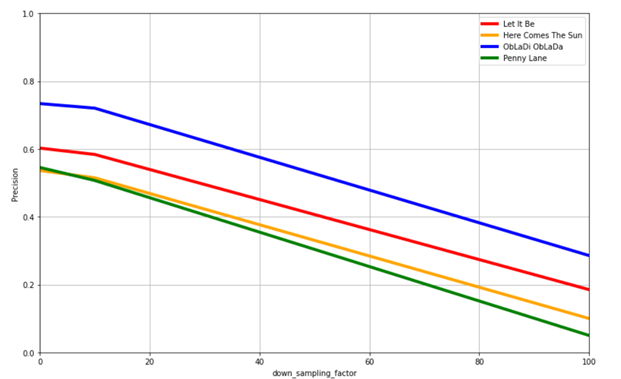
\includegraphics[scale=1]{./images/5_down_sampling_precision.png}
 \caption{Downsampling factor}
\end{figure}

\subsection*{STFT window length}

As a last test parameter we took into consideration the length of the window used for the STFT of the audio signal. We considered the values [2048, 8192, 32768] that at the default sample rate ($F_s=22050$) correspond to a small (\emph{92ms}), medium (\emph{372ms}) and large (\emph{1486ms}) window sizes. Using an analysis window with a short duration, each chroma frame contains the onsets of at most one note. Even though the sound of each note may last much longer than the notated duration, the harmonic content of each frame is dominated by only one or two notes. This explains the misclassifications and many chord label changes in the recognition result of the first setting.\\
An obvious strategy for improving the chord recognition result is to use larger window sizes. Anyway, the larger analysis windows smooth out the originally sharp transitions between different chords, which may introduce problems at chord changes.

\begin{figure}[H]
 \centering
 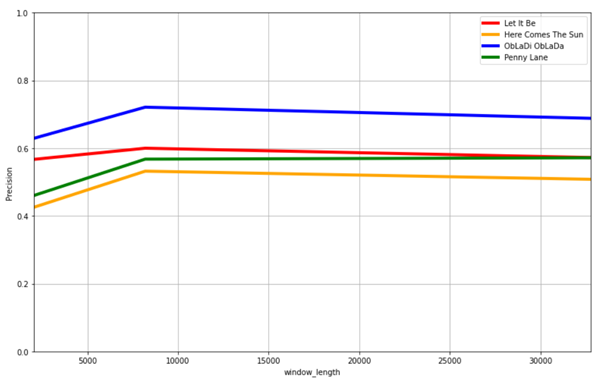
\includegraphics[scale=1]{./images/5_window_precision.png}
 \caption{Window length}
\end{figure}

%----------------------------------------------------------------------------------------

\end{document}
